\documentclass[11pt,a4paper]{article}

\usepackage[T1]{fontenc}
\usepackage[utf8]{inputenc}
\usepackage[brazil]{babel}
\usepackage{newtxtext,newtxmath}
\usepackage[a4paper,top=2.8cm,bottom=2.8cm,left=2.8cm,right=2.8cm]{geometry}
\usepackage{amsmath}
\usepackage{booktabs}
\usepackage{tabularx}
\usepackage{enumitem}
\usepackage{graphicx}
\usepackage{float}
\usepackage[font=small,labelfont=bf]{caption}
\usepackage{microtype}
\usepackage[hyphens]{url}
\usepackage{xcolor}
\definecolor{azuldoi}{rgb}{0.15,0.25,0.6}
\definecolor{fundo}{rgb}{0.95,0.95,0.93}
\usepackage[colorlinks=true,linkcolor=black,citecolor=black,urlcolor=azuldoi]{hyperref}

\setlength{\parindent}{1.5em}
\setlength{\parskip}{0.3em}
\renewcommand{\arraystretch}{1.15}
\graphicspath{{../dados/derivados/validacao/artigo/figuras/}}

\newenvironment{simbolos}
  {\begin{description}[style=nextline,leftmargin=2.6em,labelindent=0pt,font=\normalfont,itemsep=0.25em]}
  {\end{description}}

\newcommand{\Cllm}{\hat{C}^{LLM}_t}
\newcommand{\Ckf}{\hat{C}^{KF}_t}
\newcommand{\Et}{\widetilde{E}_t}

\begin{document}

\begin{center}
  {\LARGE\bfseries Um Índice de Credibilidade do Banco Central\\[0.15em]
  Baseado em Modelos de Linguagem\par}
  \vspace{0.8em}
  {\large Metodologia e resultados do índice v1.1 com o corpus ampliado\par}
  \vspace{1.2em}
  Versão de 22 de outubro de 2026 --- \textbf{antes do V-min completo}\par
  \vspace{0.6em}
\end{center}
\hrule
\vspace{1em}

\noindent\colorbox{fundo}{\parbox{\dimexpr\textwidth-2\fboxsep}{\small
\textbf{Estado desta versão.} Todos os resultados abaixo usam o corpus final
(11 veículos, 2011--2026), o pré-filtro retreinado e as notas completas do Sabiá
e do Gemini. A única parte provisória é a banda de vazamento V-max/V-min
(Seção~\ref{sec:vazamento}), que ainda usa a amostra aleatória de 9 mil notícias
da produção anterior. O V-min de todas as notícias com sinal está rodando; a
próxima versão deste documento substitui a Seção~\ref{sec:vazamento} e as
figuras correspondentes. Os critérios de aprovação foram registrados antes de
rodar (contexto do projeto, seções 4.2.17 e 4.2.20).}}

\section{Pergunta e conceito}

A credibilidade do banco central é o peso de ancoragem $C_t\in[0,1]$ que os
agentes atribuem à meta ao formar expectativas, contra $(1-C_t)$ atribuído à
inflação passada (Bomfim e Rudebusch, 2000):
\begin{equation}
  \Et[\pi_{t+1}] = C_t\,\pi^*_t+(1-C_t)\,\pi_{t-1}.
\end{equation}
Ela é latente. As medidas usuais ou derivam a credibilidade das próprias
expectativas, o que torna circular qualquer validação, ou são índices
institucionais lentos. Este projeto mede a \emph{credibilidade percebida}: o
que a imprensa econômica escreve sobre o Banco Central do Brasil (BCB), lido
por um modelo de linguagem (LLM) com um instrumento fixo. A pergunta é:

\begin{quote}
\itshape Um índice de credibilidade extraído por LLM da percepção de
terceiros sobre o BCB (i) acompanha as medidas de credibilidade implícitas nas
expectativas e nos preços, (ii) contém informação além da inflação corrente e
(iii) antecipa a ancoragem das expectativas, além do que elas já contêm?
\end{quote}

O índice é extraído da \textbf{credibilidade-resposta} (o que a audiência
acredita), e não do \textbf{esforço de sinalização} do BCB. Por isso o corpus é
texto \emph{sobre} o BCB escrito por terceiros, e declarações do BCB
reproduzidas numa matéria pesam pelo enquadramento que o veículo lhes dá.

\section{Corpus}\label{sec:corpus}

\paragraph{Veículos e período.} Matérias de janeiro de 2011 a agosto de 2026
em 11 veículos (Figura~\ref{fig:cobertura}). Os cinco do corpus original
(Valor, O Globo, InfoMoney, Money Times, Poder360) foram ampliados com Exame,
G1, CartaCapital, Bloomberg Línea, Agência Brasil e Folha. O corpus final tem
110.279 notícias; 10\% delas, separadas pelo \emph{hash} do identificador, ficam
em quarentena fora da produção (Seção~\ref{sec:pesquisador}).

\paragraph{Coleta.} Termos específicos de política monetária (\emph{Copom},
\emph{Selic}, \emph{ata do Copom}, \emph{política monetária}, \emph{meta de
inflação}, \emph{Relatório de Inflação}, \emph{Banco Central}), com um filtro
temático local que exige um deles no título, na linha fina ou no primeiro
parágrafo. Cada veículo usa o canal que o próprio site oferece:
\begin{itemize}[leftmargin=1.5em,itemsep=0.1em]
  \item busca da Globo (Valor, O Globo, G1; no G1, um plano fixo de 65 consultas,
  porque a busca não ordena por data);
  \item API REST do WordPress, por ano (InfoMoney, Money Times, Poder360, Exame,
  CartaCapital); a paginação para no total informado pelo próprio site;
  \item sitemaps diários (Bloomberg Línea, desde julho de 2021) e listagem da
  seção Economia (Agência Brasil, 10 s entre requisições como pede o site),
  com pré-filtro pelas palavras do endereço;
  \item a Folha foi coletada pela equipe com coletor próprio, sob autorização
  da FEA, e cobre 2018 em diante.
\end{itemize}
Valor e O Globo são coletados sob acesso concedido à equipe. A listagem da
Agência Brasil só alcança janeiro de 2014; a seção Política ficou de fora.

\paragraph{Unidade e deduplicação.} Cada item é título, linha fina e primeiro
parágrafo. A mesma URL conta uma vez; a mesma matéria em duas URLs, no mesmo
veículo e dia, também. Matérias de agência replicadas em vários veículos formam
um \emph{cluster} e contam uma vez por mês. A data é a hora local de Brasília.

\begin{figure}[H]
  \centering
  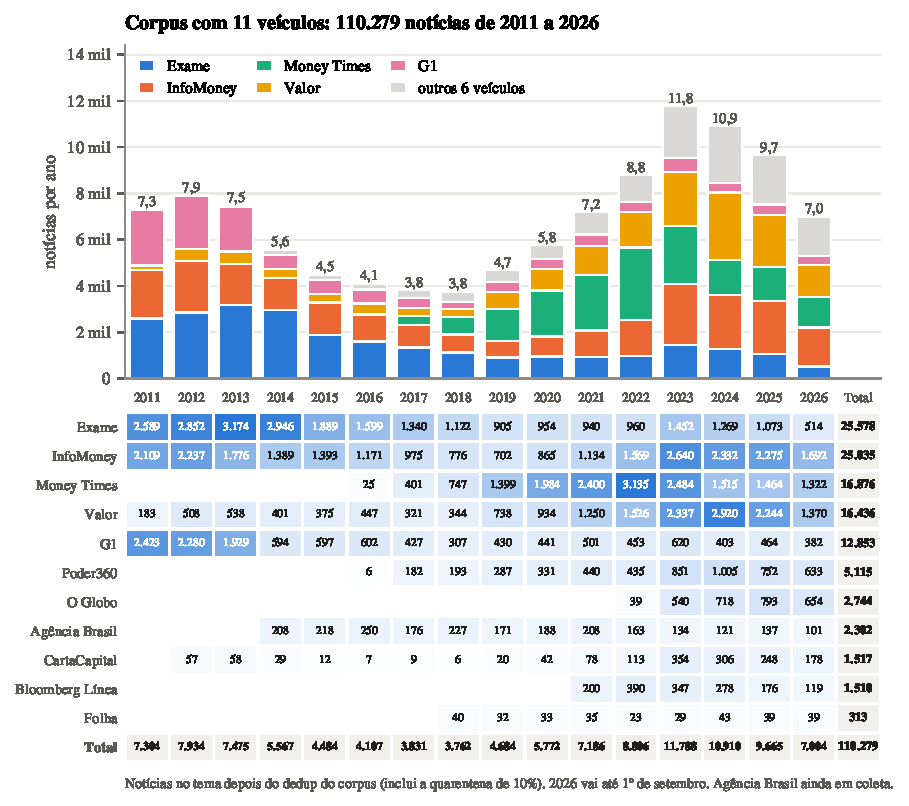
\includegraphics[width=\textwidth]{fig02_cobertura_veiculos.pdf}
  \caption{Notícias por veículo e ano no corpus final. Barras: os cinco maiores
  veículos em cor e os demais em cinza; tabela: todos os veículos, com totais.}
  \label{fig:cobertura}
\end{figure}

\paragraph{Uso dos dados.} O texto das matérias é de terceiros e não é
redistribuído. São públicos apenas agregados, contagens e identificadores
opacos.

\section{Instrumento}

Cada notícia é lida, uma por chamada, por um LLM com prompt de sistema fixo
(v1.1, \emph{hash} \texttt{c4cd8123f2832031}), temperatura zero e saída JSON.
Três dimensões, em escalas de 1 a 5 com âncoras:
\begin{simbolos}
  \item[D1] \textbf{probabilidade percebida de cumprimento da meta}. O modelo
  decide primeiro se há sinal sobre o cumprimento; sem sinal, não há nota.
  Com sinal: 1 = descumprimento certo, 3 = equilibrado, 5 = cumprimento certo.
  \item[D2] confiança na condução da política monetária (diagnóstica).
  \item[D3] autonomia percebida frente ao governo (diagnóstica).
\end{simbolos}
O índice usa só a D1. O prompt manda avaliar a percepção que o texto transmite,
separa pessimismo macroeconômico de descrédito na autoridade monetária, conta
ironia e escolha de fontes céticas como sinal e pede que o modelo se comporte
como na data de publicação. A v1.1 difere da v1.0 numa única regra: separa
``sem sinal'' de ``equilibrado'', que a v1.0 juntava na nota 3.

\paragraph{Modelos.} Série principal: Sabiá (Maritaca AI, \emph{sabiazinho-4}).
Robustez: Gemini 3.1 Flash-Lite (Google) nas mesmas notícias. O Gemini foi
pontuado pela API de lote, com a mesma requisição da chamada individual; num
teste com 30 notícias com sinal, as notas de D1, D2 e D3 foram idênticas nas
duas vias. Várias notícias por chamada foram testadas e rejeitadas: a nota de
uma notícia passa a depender das outras do lote.

\section{Do item ao índice}\label{sec:agregacao}

Para cada item $i$ com sinal na D1, $c_i=(d_{1,i}-1)/4\in[0,1]$. Com o
\emph{cluster} de agência colapsado em uma observação $k$ por mês, o efeito de
tipo de veículo é estimado em $c_{kt}=\alpha_t+\gamma_{v(k)}+e_{kt}$ e o índice
mensal é a média dos itens ajustados,
\begin{equation}
  \Cllm = \frac{1}{N_t}\sum_{k\in S_t}\bigl(c_{kt}-\hat\gamma_{v(k)}\bigr),
\end{equation}
com erro-padrão agrupado por dia. A regra registrada antes da validação reporta
duas séries: a mensal e a janela móvel de três meses para trás, que soma itens
de $t-2$ a $t$. O índice diário serve ao estudo de eventos; D2 e D3 usam a
média ponderada pelo desenho do pré-filtro.

\section{Pré-filtro de sinal com auditoria aleatória}\label{sec:filtro}

A maior parte das notícias não traz sinal sobre a meta. Um classificador local
(BERTimbau, Souza, Nogueira e Lotufo, 2020) decide o que vai à API, e uma
auditoria aleatória mede o que se perde.

\begin{enumerate}[leftmargin=2em,itemsep=0.15em]
  \item \textbf{Rotulagem.} Uma amostra aleatória da produção é pontuada
  inteira pela API: 9.000 notícias do corpus original e 15\% das notícias
  novas, sorteadas pelo \emph{hash} do identificador (6.017).
  \item \textbf{Filtro único.} O BERTimbau é treinado uma vez, com os rótulos
  do Sabiá das duas amostras (11.997 para treino, 2.999 para validação), e
  vale para o corpus inteiro. Metade da validação escolhe o limiar para
  sensibilidade de pelo menos 95\%; a outra metade mede a sensibilidade.
  \item \textbf{Roteamento.} Vai à API o que passa do limiar e, por sorteio,
  10\% das descartadas (auditoria). Notas já existentes são reaproveitadas.
\end{enumerate}

\noindent O filtro tem AUC de 0,981 e sensibilidade de 95,3\% na metade de
teste (limite inferior de 92,2\%, Clopper--Pearson unilateral a 95\%), com 74\%
das notícias descartadas. Por veículo (Tabela~\ref{tab:sens}), a sensibilidade
fica entre 97\% e 100\%, exceto Exame (91\%) e Valor (89\%); com 35 e 54
positivos, os intervalos são largos. Valor fica abaixo do patamar de 90\%
registrado e entra nas limitações.

\begin{table}[H]
\centering\small
\caption{Sensibilidade do filtro por veículo, na metade de teste.}\label{tab:sens}
\begin{tabular}{@{}lrrr@{}}
\toprule
Veículo & Positivos & Sensibilidade & Limite inferior 95\% \\
\midrule
Valor & 54 & 0,889 & 0,79 \\
Exame & 35 & 0,914 & 0,79 \\
Money Times & 34 & 0,971 & 0,87 \\
G1 & 32 & 1,000 & 0,91 \\
InfoMoney & 30 & 1,000 & 0,90 \\
Poder360 & 11 & 1,000 & 0,76 \\
CartaCapital, Ag.\ Brasil, Línea, O Globo, Folha & 17 & 1,000 & --- \\
\bottomrule
\end{tabular}
\end{table}

\begin{table}[H]
\centering\small
\caption{Contagens do corpus à série (Sabiá).}\label{tab:contagens}
\begin{tabular}{@{}lr@{}}
\toprule
Corpus & 110.279 \\
Quarentena (fora da produção) & 11.033 \\
Produção & 99.246 \\
\quad rotulagem (inteira à API) & 15.017 \\
\quad enviadas pelo filtro & 22.438 \\
\quad descartadas e auditadas (à API) & 6.179 \\
\quad descartadas não enviadas (56,0\% da produção) & 55.612 \\
Notas da API sem sinal na D1 & 29.733 \\
Notas da API com sinal na D1 & 13.901 \\
Taxa de sinal na auditoria & 0,73\% \\
Sinal perdido estimado & $\approx$ 405 notícias (2,8\% do sinal) \\
Erros da API & 0 \\
\bottomrule
\end{tabular}
\end{table}

\noindent Pelo critério do Gemini, a auditoria encontra mais sinal nas
descartadas (2,2\%), o que dá 6,3\% de sinal perdido; com o filtro anterior
eram 13\%. Como robustez, o índice com pesos de Horvitz e Thompson (1952) na
forma de Hájek (peso 10 para as auditadas) tem correlação de 0,996 com o
índice simples.

\begin{figure}[H]
  \centering
  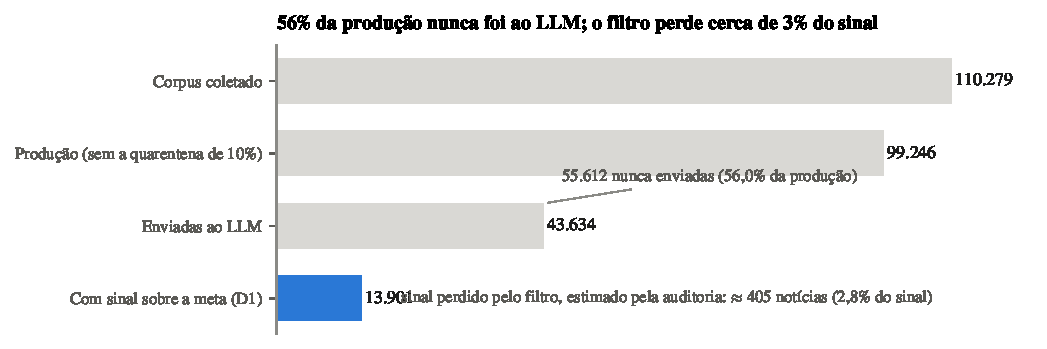
\includegraphics[width=\textwidth]{fig01_funil_corpus.pdf}
  \caption{Do corpus às notícias com sinal sobre a meta.}
\end{figure}

\section{Resultados: o índice}

\begin{figure}[H]
  \centering
  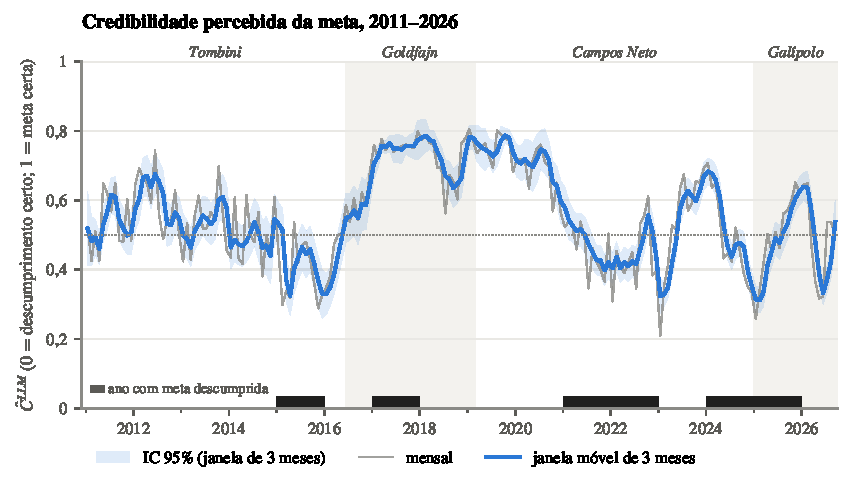
\includegraphics[width=\textwidth]{fig03_indice.pdf}
  \caption{Índice mensal e janela móvel de três meses (Sabiá), com a meta e as
  gestões do BCB.}
  \label{fig:indice}
\end{figure}

O índice mensal tem média 0,559 e desvio-padrão 0,139. O máximo é janeiro de
2019 (0,80) e o mínimo, janeiro de 2023 (0,21). Por gestão: Tombini 0,51,
Goldfajn 0,71, Campos Neto 0,56 e Galípolo 0,49 (até agosto de 2026). A
mediana de notícias com sinal por mês é 63 (8 meses com menos de 20); na janela
de três meses, 185 (mínimo de 51). O erro-padrão mensal médio é 0,044.

A ampliação do corpus muda pouco a série e muito a sua precisão: contra o
índice do corpus original, a correlação é 0,958 e a diferença média, $-0{,}007$,
enquanto as notícias com sinal por mês praticamente dobram. Sabiá e Gemini
têm correlação de 0,942 (mensal) e 0,962 (janela de três meses); o Gemini fica
em média 0,03 acima.

\begin{figure}[H]
  \centering
  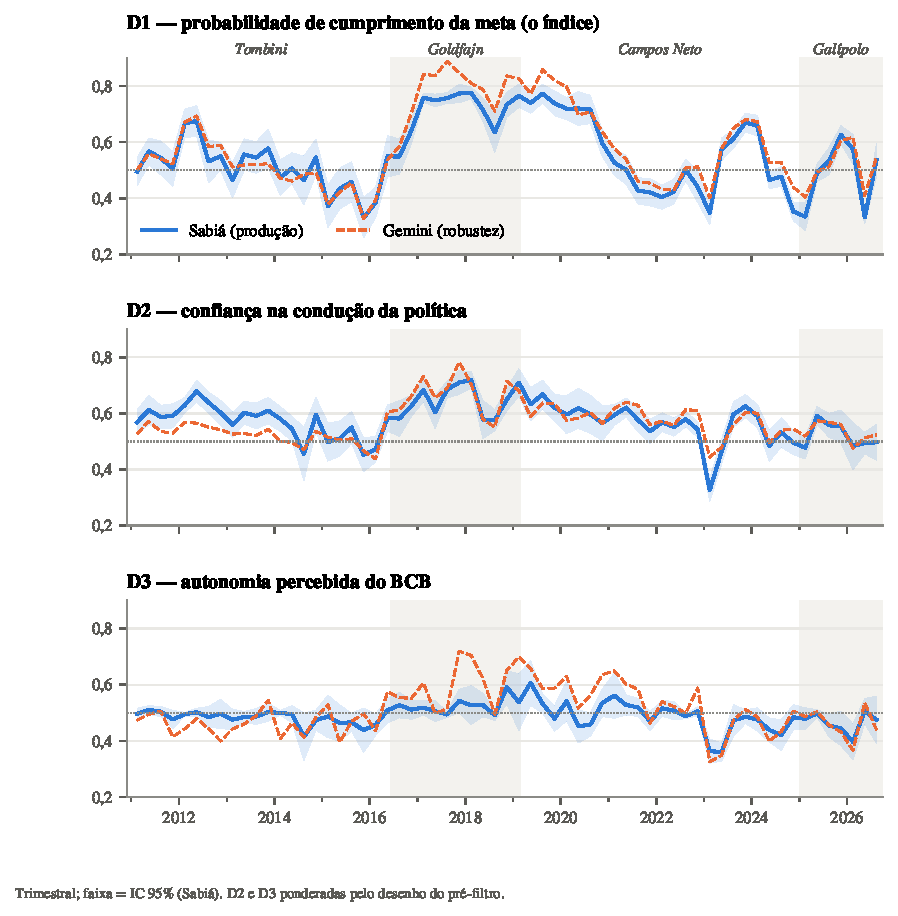
\includegraphics[width=\textwidth]{fig04_dimensoes.pdf}
  \caption{D1, D2 e D3 (Sabiá e Gemini). D2 e D3 são diagnósticas.}
\end{figure}

\section{Robustez da construção}\label{sec:robustez}

Todas as versões são reagregações das notas existentes, sem chamadas novas.

\begin{table}[H]
\centering\small
\caption{Correlação com o índice principal (mensal; entre parênteses, janela de três meses).}\label{tab:robustez}
\begin{tabular}{@{}lcc@{}}
\toprule
Versão & Correlação & Notícias com sinal/mês \\
\midrule
Efeito fixo por veículo & 0,998 (0,998) & 64 \\
Só veículos presentes em toda a série & 0,983 (0,997) & 49 \\
Só os 5 veículos originais & 0,955 (0,985) & 30 \\
Só InfoMoney & 0,911 (0,957) & 12 \\
Só Valor & 0,803 (0,889) & 13 \\
Só a amostra aleatória (sem filtro) & 0,857 (0,954) & 10 \\
Sem Exame / sem G1 & 0,989 / 0,993 & 45 / 49 \\
Sem Agência Brasil, Línea, CartaCapital ou Folha & $\ge 0{,}999$ & 60--63 \\
Outro modelo (Gemini) & 0,942 (0,962) & --- \\
\bottomrule
\end{tabular}
\end{table}

\noindent Nenhuma fonte nova sozinha move o índice: retirar qualquer uma
mantém correlação de pelo menos 0,989. A versão sem o filtro (só a amostra
aleatória) acompanha a principal na janela de três meses (0,954); no mensal,
a correlação menor reflete as 10 notícias com sinal por mês.

\begin{figure}[H]
  \centering
  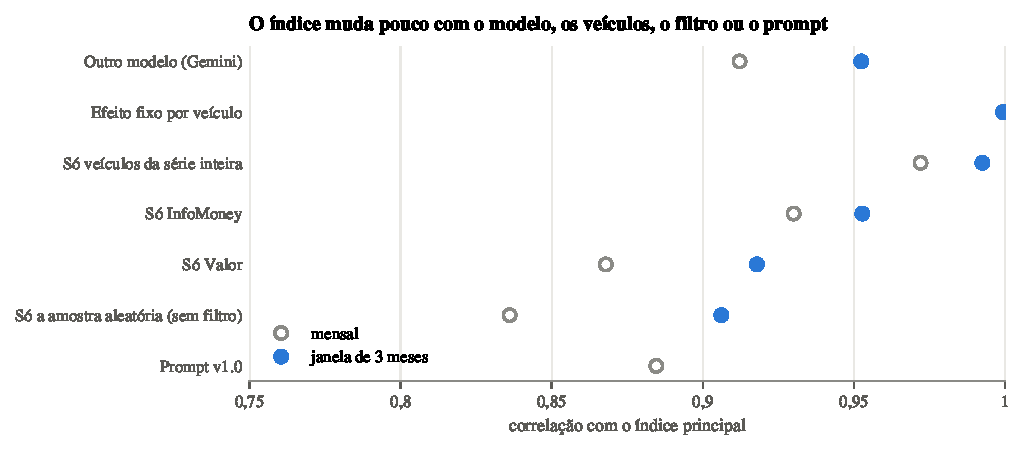
\includegraphics[width=\textwidth]{fig05_robustez.pdf}
  \caption{Correlação do índice principal com versões alternativas.}
\end{figure}

\section{Vazamento temporal}\label{sec:vazamento}

Nenhum LLM de fronteira é temporalmente cego. O desenho limita o vazamento por
construção (trecho curto, âncoras explícitas, restrição temporal no prompt),
mede-o e o reporta.

\subsection{Vazamento do pesquisador}\label{sec:pesquisador}

O prompt é congelado e identificado por \emph{hash}; 10\% do corpus fica em
quarentena; critérios e regras de agregação são registrados antes de rodar;
revisões posteriores são declaradas. A revisão v1.0$\to$v1.1, a regra da
janela de três meses e o desenho das fontes novas foram registrados antes dos
resultados que dependiam deles.

\subsection{Bateria de testes}

\begin{table}[H]
\centering\small
\caption{Bateria anti-vazamento (registrada antes de rodar).}
\begin{tabularx}{\textwidth}{@{}l X l@{}}
\toprule
Teste & Resultado & Veredito \\
\midrule
T0 (datar o texto, L1--L5) & o modelo data o texto mesmo mascarado (erro de 1,6 a 3,3 anos) & reprova \\
T2 (data omitida/trocada) & nota muda em 3--4\% das notícias; $\rho$ com a surpresa futura $\le 0{,}10$ ($p\ge 0{,}24$) & passa \\
T3 (anonimização L1--L4) & muda em 1--5\%; L4 com $\rho=0{,}20$ ($p=0{,}02$) apoiado em 2 notícias & passa, frágil \\
T4 (resíduo V-max sobre V-min) & coeficiente $-0{,}001$ ($p=0{,}68$) & passa \\
T5 (pares sintéticos) & diferença pareada 0,00 & passa \\
T6 (encoder local, pós-2019) & correlação BERTimbau $\times$ Sabiá 0,94 antes e depois de 2019 & sem sinal \\
\bottomrule
\end{tabularx}
\end{table}

\noindent O T0 é condição suficiente, não necessária: o modelo sabe datar o
texto, mas omitir, trocar ou mascarar a data e os identificadores quase não
muda a nota, e o que muda não se correlaciona com o desfecho futuro (T2--T5).

\subsection{Banda V-max/V-min (provisória)}

A V-min repontua as notícias no nível L5 (sem números, nomes, termos de época
e veículo). Ela é reportada como \emph{limite inferior} da informação do
índice, não como veto: o L5 retira também os números de inflação, que são
evidência legítima da D1. \textbf{Nesta versão}, a banda usa a amostra
aleatória de 9 mil notícias do corpus original (cerca de 7 notícias com sinal
por mês): correlação mensal V-max $\times$ V-min de 0,80 em 175 meses e
$\Delta_t$ médio de $+0{,}014$ (desvio de 0,10). A próxima versão usa o V-min
de todas as notícias com sinal (registro 4.2.20), com precisão muito maior.

\begin{figure}[H]
  \centering
  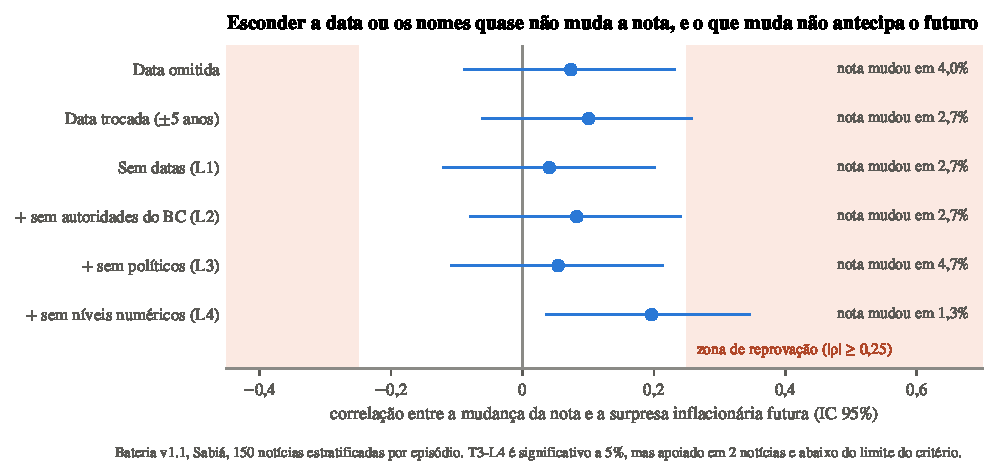
\includegraphics[width=\textwidth]{fig06_vazamento.pdf}
  \caption{Notas com a data e os nomes escondidos (V-min) contra o texto
  inteiro (V-max). Provisória: amostra de 9 mil notícias.}
\end{figure}

\section{Validação: validade de construto}\label{sec:validacao}

Sem gabarito observável, o índice é defendido por uma bateria com critérios
registrados antes de rodar (Baker, Bloom e Davis, 2016). Toda variável é
orientada como ``maior = mais credibilidade''; erros de Newey e West (1987) com
$h+\lfloor 4(n/100)^{2/9}\rfloor$ defasagens. Série principal: Sabiá mensal.
As séries de fornecedor (EMBI+, CDS) entram nas regressões, mas não são
publicadas.

\begin{table}[H]
\centering\small
\caption{Vereditos da bateria (Sabiá mensal).}\label{tab:vereditos}
\begin{tabularx}{\textwidth}{@{}l X l@{}}
\toprule
Teste & Critério registrado & Resultado \\
\midrule
7.1 Convergente & correlação positiva, $p<5\%$, com o \emph{breakeven} e com uma medida do Focus & \textbf{aprovado} \\
7.2 Discriminante & $R^2$ da inflação $<0{,}8$ e $c>0$, $p<5\%$, para \emph{breakeven} ou EMBI+ & \textbf{aprovado} \\
7.3 Preditiva & $b>0$, $p<5\%$, para a distância do Focus à meta em $h=6$ & \textbf{aprovado} \\
7.4 \emph{Encompassing} & --- (reportado) & sobrevive a 5 de 9 rivais \\
\bottomrule
\end{tabularx}
\end{table}

\subsection{Convergente}

\begin{table}[H]
\centering\small
\caption{Correlação do índice com as medidas do painel (valor-p HAC).}\label{tab:conv}
\begin{tabular}{@{}lcc@{}}
\toprule
Medida & Mensal & Janela de 3 meses \\
\midrule
Distância do Focus à meta (sinal invertido) & 0,75 (0,00) & 0,84 (0,00) \\
Inflação implícita de 5 anos (sinal invertido) & 0,74 (0,00) & 0,79 (0,00) \\
de Mendonça (2007) & 0,68 (0,00) & 0,76 (0,00) \\
Dispersão do Focus (sinal invertido) & 0,57 (0,00) & 0,63 (0,00) \\
de Mendonça e Souza (2009) & 0,44 (0,00) & 0,51 (0,00) \\
Latente do Kalman & 0,38 (0,00) & 0,42 (0,00) \\
CDS (sinal invertido; desde 2019) & 0,22 (0,21) & 0,23 (0,23) \\
Inclinação da curva & 0,18 (0,10) & 0,27 (0,01) \\
EMBI+ (sinal invertido) & 0,13 (0,37) & 0,13 (0,41) \\
\bottomrule
\end{tabular}
\end{table}

\begin{figure}[H]
  \centering
  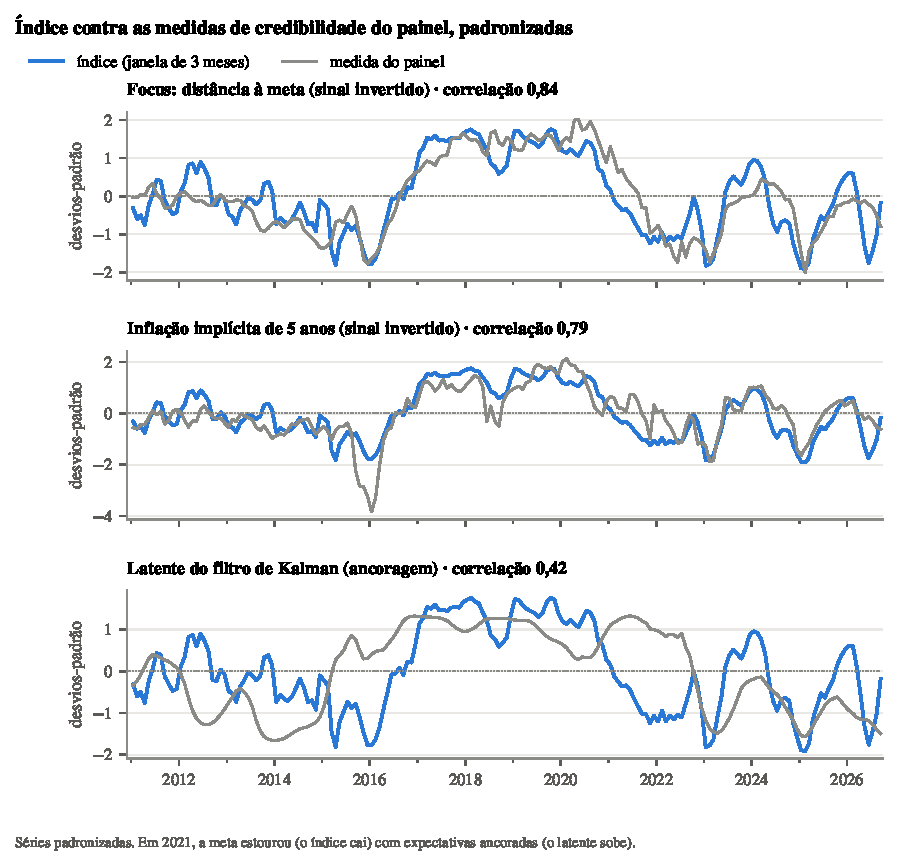
\includegraphics[width=\textwidth]{fig07_convergencia.pdf}
  \caption{Índice contra o Focus, a inflação implícita e o latente do Kalman.}
\end{figure}

\subsection{Discriminante}

A inflação corrente (desvio da meta, variação em 12 meses e estouro do teto)
explica 42\% da variância do índice mensal; o restante vem do texto
(Figura~\ref{fig:alem}). Controlando por inflação, o índice padronizado explica
a inflação implícita ($c=0{,}48$, $p<0{,}001$) e a distância do Focus à meta
($c=0{,}45$, $p<0{,}001$). Com o EMBI+ o coeficiente é \emph{negativo}
($c=-16$, $p=0{,}02$): dada a inflação, meses de maior credibilidade percebida
coincidem com risco-país maior. O EMBI+ carrega risco fiscal e global que a D1
não mede; o resultado vai para a discussão, não para o critério, que já é
cumprido pelo \emph{breakeven}.

\begin{figure}[H]
  \centering
  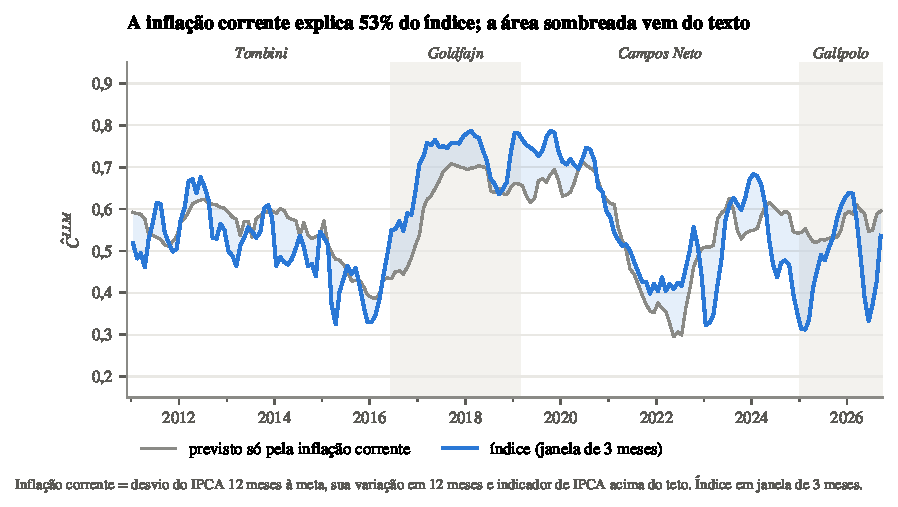
\includegraphics[width=\textwidth]{fig08_alem_da_inflacao.pdf}
  \caption{Parte do índice explicada pela inflação corrente e parte que vem
  do texto.}\label{fig:alem}
\end{figure}

\subsection{Preditiva}

\begin{equation}
  y_{t+h}-y_t = a + b\,z(\Cllm) + c\,y_t + d\,\Delta y_t + e\,g_t + \varepsilon_{t+h}.
\end{equation}
Primário: distância do Focus à meta em $h=6$, $b=0{,}30$ ($p=0{,}003$; Holm
$0{,}009$). O índice também antecipa o Focus em 1 e 3 meses. A inflação
implícita tem $b=0{,}28$ ($p=0{,}03$) em $h=6$, que não sobrevive à correção de
Holm ($0{,}07$) no mensal e sobrevive na janela de três meses ($0{,}05$) e no
Gemini ($0{,}001$). O EMBI+ não é antecipado em nenhum horizonte.

\begin{figure}[H]
  \centering
  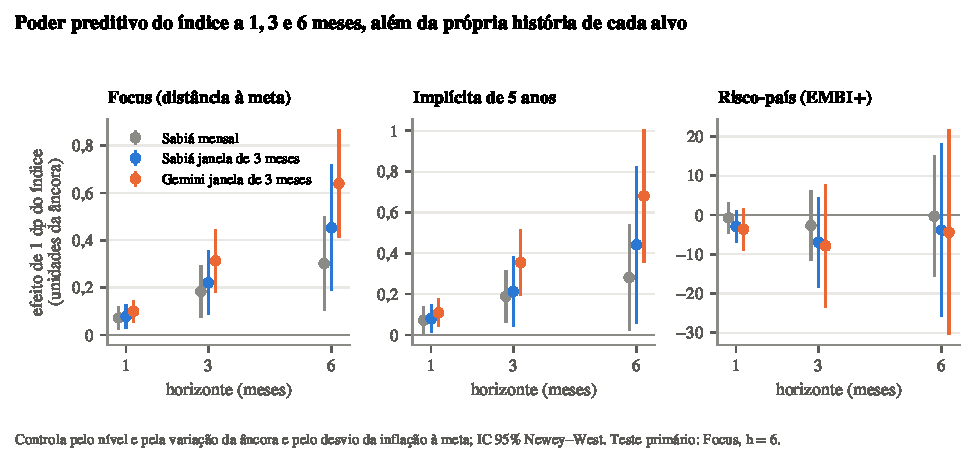
\includegraphics[width=\textwidth]{fig09_preditiva.pdf}
  \caption{Coeficiente do índice na previsão de cada alvo a 1, 3 e 6 meses.}
\end{figure}

\subsection{\emph{Encompassing} contra o latente do Kalman}

O latente $\Ckf$ vem só do Focus, da meta e do IPCA defasado, num modelo de
parâmetro variável no tempo com elo logístico, estimado por filtro de Kalman
estendido. Sozinho, o índice explica o latente ($b_1=0{,}38$, $p=0{,}001$,
$R^2=0{,}15$) e continua significativo com 5 dos 9 rivais (de Mendonça e Souza,
dispersão do Focus, CDS, EMBI+ e inclinação). Perde significância com de
Mendonça (2007), com a inflação implícita e com todos os rivais juntos. Os dois
objetos não coincidem por construção: $\Ckf$ mede quanto o Focus fica perto da
meta apesar da inflação passada, e a D1, se a meta será cumprida. Em 2021 a
meta estourou, o índice caiu e o latente subiu.

\section{Aplicação: estudo de eventos}\label{sec:eventos}

\paragraph{Reuniões do Copom.} $\Delta_m=\bar c_{[D+1,D+7]}-\bar c_{[D-7,D-1]}$
regredido na surpresa do swap DI$\times$Pré de 3 meses (B3) de $D-1$ a $D+1$,
erro HC1. O teste primário (7 dias) não é significativo: $+0{,}009$ por 10 pb
($p=0{,}42$, 115 reuniões). Na janela de 14 dias, secundária, o efeito é
$+0{,}019$ por 10 pb ($p=0{,}007$): surpresas de aperto elevam a credibilidade
percebida nas duas semanas seguintes. O tamanho da surpresa, sem sinal, não
tem efeito.

\begin{figure}[H]
  \centering
  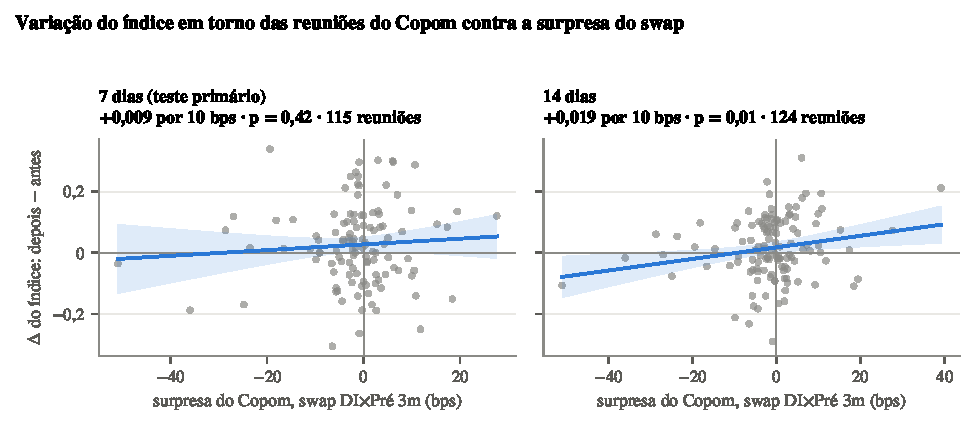
\includegraphics[width=\textwidth]{fig10_copom.pdf}
  \caption{Variação do índice em torno das reuniões do Copom contra a surpresa.}
\end{figure}

\paragraph{Eventos institucionais (exploratório).} Variação de D1, D2 e D3 em
$\pm30$ dias, contra a distribuição placebo de todas as datas. Nenhum evento sai
da faixa de 5\%. Os maiores, na D1: anúncio da diretoria de Goldfajn e da
proposta de autonomia técnica em maio de 2016 ($+0{,}13$; 16\% das datas placebo
têm variação maior), críticas presidenciais à autonomia em janeiro de 2023
($+0{,}15$; 10\%) e a decisão dividida do Copom em maio de 2024 ($-0{,}13$; 16\%).
A alta de janeiro de 2023 parte do mínimo da série, em meio às notícias de
estouro da meta de 2022.

\begin{figure}[H]
  \centering
  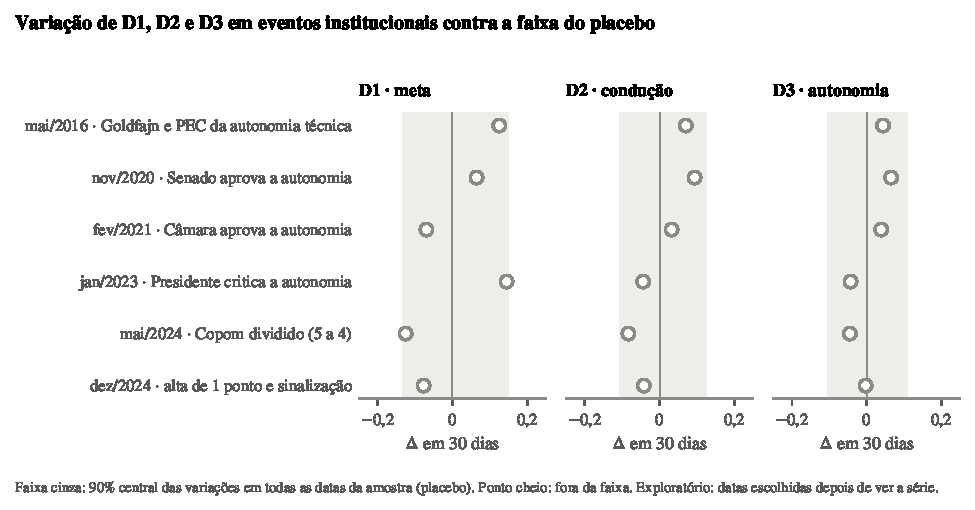
\includegraphics[width=\textwidth]{fig11_eventos_institucionais.pdf}
  \caption{Variação de D1, D2 e D3 nos eventos institucionais e faixa placebo.}
\end{figure}

\section{Limitações}

\begin{enumerate}[leftmargin=2em,itemsep=0.15em]
  \item \textbf{Composição do corpus.} O G1 concentra-se em 2011--2013 (cerca de
  3 mil notícias por ano, contra 300--600 depois); a Agência Brasil começa em
  2014, a Bloomberg Línea em 2021 e a Folha em 2018. O efeito fixo por veículo
  e as versões ``sem a fonte'' mostram efeito pequeno no índice.
  \item \textbf{Filtro.} Sensibilidade de 89\% no Valor e 91\% na Exame, com
  intervalos largos; o sinal perdido é estimado pela auditoria e corrigido no
  IPW, mas não na série principal de D1.
  \item \textbf{Cobertura das fontes por endereço.} Línea e Agência Brasil usam
  pré-filtro pelas palavras do endereço; matérias cujo endereço não traz os
  termos escapam.
  \item \textbf{Vazamento.} O modelo data o texto (T0). A evidência de que a
  nota não usa o futuro vem de T2--T5; a banda V-min desta versão é imprecisa.
  \item \textbf{Âncoras.} A inflação implícita contém prêmios de risco e de
  liquidez; o EMBI+ e o CDS carregam risco fiscal e global.
  \item \textbf{Quarentena congelada tarde.} O manifesto foi gerado depois de
  a série ter sido inspecionada; as séries mudaram pouco (correlação 0,997).
\end{enumerate}

\section{Custo e reprodução}

As chamadas desta rodada (fontes novas, filtro único, Sabiá individual e Gemini
em lote) custaram cerca de R\$~50, estimados pelas chamadas registradas
(23.819 no Sabiá, 23.818 no Gemini em lote); o V-min acrescenta cerca de R\$~10.
O código e as séries estão no repositório; a sequência é
\texttt{coleta/} $\to$ \texttt{llm/corpus/from\_coleta.py} $\to$
\texttt{llm/producao\_v11.py} (rotulagem, filtro, roteamento, pontuação,
V-min, consolidação) $\to$ \texttt{python -m validacao.artigo}.

\section*{Referências}
{\small
\begin{list}{}{\setlength{\leftmargin}{1.5em}\setlength{\itemindent}{-1.5em}\setlength{\itemsep}{0.3em}}
\item BAKER, S. R.; BLOOM, N.; DAVIS, S. J. Measuring economic policy uncertainty. \emph{The Quarterly Journal of Economics}, v. 131, n. 4, p. 1593--1636, 2016.
\item BOMFIM, A. N.; RUDEBUSCH, G. D. Opportunistic and deliberate disinflation under imperfect credibility. \emph{Journal of Money, Credit and Banking}, v. 32, n. 4, p. 707--721, 2000.
\item DE MENDONÇA, H. F. Towards credibility from inflation targeting: the Brazilian experience. \emph{Applied Economics}, v. 39, n. 20, p. 2599--2615, 2007.
\item DE MENDONÇA, H. F.; GUIMARÃES E SOUZA, G. J. Inflation targeting credibility and reputation: the consequences for the interest rate. \emph{Economic Modelling}, v. 26, n. 6, p. 1228--1238, 2009.
\item HOLM, S. A simple sequentially rejective multiple test procedure. \emph{Scandinavian Journal of Statistics}, v. 6, n. 2, p. 65--70, 1979.
\item HORVITZ, D. G.; THOMPSON, D. J. A generalization of sampling without replacement from a finite universe. \emph{Journal of the American Statistical Association}, v. 47, n. 260, p. 663--685, 1952.
\item KALMAN, R. E. A new approach to linear filtering and prediction problems. \emph{Journal of Basic Engineering}, v. 82, n. 1, p. 35--45, 1960.
\item KUTTNER, K. N. Monetary policy surprises and interest rates: evidence from the Fed funds futures market. \emph{Journal of Monetary Economics}, v. 47, n. 3, p. 523--544, 2001.
\item NEWEY, W. K.; WEST, K. D. A simple, positive semi-definite, heteroskedasticity and autocorrelation consistent covariance matrix. \emph{Econometrica}, v. 55, n. 3, p. 703--708, 1987.
\item SOUZA, F.; NOGUEIRA, R.; LOTUFO, R. BERTimbau: pretrained BERT models for Brazilian Portuguese. In: \emph{Brazilian Conference on Intelligent Systems (BRACIS)}. Cham: Springer, 2020. p. 403--417.
\end{list}
}

\end{document}
